\documentclass[12pt,a4paper]{article}
\usepackage[utf8]{inputenc}
\usepackage[russian]{babel}
\usepackage[OT1]{fontenc}
\usepackage{amsmath}
\usepackage{amsfonts}
\usepackage{amssymb}
\usepackage{graphicx}
\usepackage{array}
\usepackage{cancel}
\usepackage{caption}
\usepackage{wrapfig}
\usepackage{secdot}
\usepackage{indentfirst}
\usepackage[left=1.5cm,right=1.5cm,top=0.3cm,bottom=1.5cm,includefoot,footskip=1.5cm]{geometry}
\usepackage{psfrag}
\begin{document}
\textbf{
\begin{flushright}
Илья Кочергин, 626 группа
\end{flushright}}
\paragraph{\large Работа 122}
\paragraph{\Large Резонанс напряжений в последовательном контуре}
\paragraph{Цель работы:}исследование резонанса напряжений в последовательном колебательном контуре с изменяемой ёмкостью, включающее получение АЧХ и ФЧХ, а также определение основных параметров контура.
\paragraph{Оборудование:}генератор сигналов, источник напряжения, нагруженный на последовательный колебательный контур с переменной ёмкостью, двулучевой осциллограф, цифровые вольтметры.
\section{Теоретическая справка} 
\paragraph{Общие уравнения.} Рассмотрим электрическую цепь, состоящую из последовательно соединенных конденсатора с емкостью $C$ и активным сопротивлением $R_S$, катушки с индуктивностью $L$ и активным сопротивлением $R_L$ и резистора с сопротивлением $R$, которая подключена к источнику переменного тока с амплитудой напряжения $E$ и частотой $f$. Тогда общее активное сопротивление цепи $R_\Sigma$ выражается формулой
\begin{equation}
R_\Sigma = R + R_S + R_L\label{rsum},
\end{equation}
а циклическая частота $\omega$ формулой
 \begin{equation}
\omega = 2\pi f\label{omeg}.
\end{equation}
Отсюда импеданс цепи определяется выражением
\begin{equation}
Z = R_\Sigma + i\left(\omega L - \frac{1}{\omega C}\right)\label{imp},
\end{equation}
из которого можно легко найти формулу для комплексной амплитуды тока $\widehat{I}$:
\begin{equation}
\widehat{I} = \frac{\widehat{E}}{Z} = \frac{E}{R_\Sigma + i\left(\omega L - \frac{1}{\omega C}\right)}\label{Ic}.
\end{equation}
Из предыдущего выражения несложно получить формулы для комплексной амплитуды напряжения на конденсаторе $\widehat{U}_C$, а также для его амплитуды $U_C$ и сдвига фаз $\varphi_C$:
\begin{equation}
\widehat{U}_C = E\frac{R_S - \frac{i}{\omega C}}{R_\Sigma + i\left(\omega L - \frac{1}{\omega C}\right)}\label{ucc};
\end{equation}
\begin{equation}
U_C = E\sqrt{\frac{R_S^2\omega^2C^2+1}{\frac{1}{Q^2}\left(\frac{\omega}{\omega_0}\right)^2 + \left(\left(\frac{\omega}{\omega_0}\right)^2-1\right)^2}}\label{uc};
\end{equation}
\begin{equation}
\varphi_C = -\arccos\left(\frac{\frac{1}{Q}R_S\omega C - \left(\left(\frac{\omega}{\omega_0}\right)^2-1\right)^2}{\sqrt{R_S^2\omega^2+1}\sqrt{\frac{1}{Q^2}\left(\frac{\omega}{\omega_0}\right)^2 + \left(\left(\frac{\omega}{\omega_0}\right)^2-1\right)^2}}\right)\label{phic}.
\end{equation}
Здесь были использованы следующие обозначения:
\begin{equation}
\begin{cases}
\omega_0 = \frac{1}{\sqrt{LC}}\text{ - собтвенная циклическая частота контура};\\
Q = \frac{1}{R}\sqrt{\frac{L}{C}}\text{ - добротность контура}.\\ 
\end{cases}\label{redef}
\end{equation}
\paragraph{Приближение вблизи резонанса.} Видно, что выражения (\ref{uc}) - (\ref{phic}) являются достаточно громоздкими. Для их упрощения примем, что добротность контура велика ($Q \ge 10$) и $R_S \ll R$, и будем рассматривать поведение цепи вблизи резонанса. Тогда можно считать $\omega_0$ резонансной циклической частотой контура, а эти выражения примут вид:
\begin{equation}
U_C = EQ\frac{\omega}{\omega_0}\frac{1}{\sqrt{1+\left(\tau\Delta\omega\right)^2}}\label{uca};
\end{equation}
\begin{equation}
\varphi_c = -\frac{\pi}{2} + \delta - \arctg(\tau\Delta\omega)\label{pca}.
\end{equation}
Новые использованные обозначения:
\begin{equation}
\begin{cases}
\tau= \frac{2Q}{\omega_0}\text{ - постоянная времени контура};\\
\delta = \arctg(RC\omega)\text{ - параметр конденсатора (см. рис. \ref{Fig1})}.\\ 
\Delta\omega = \omega - \omega_0
\end{cases}\label{redef2}
\end{equation}
\begin{wrapfigure}{r}{0.24\textwidth}
\centering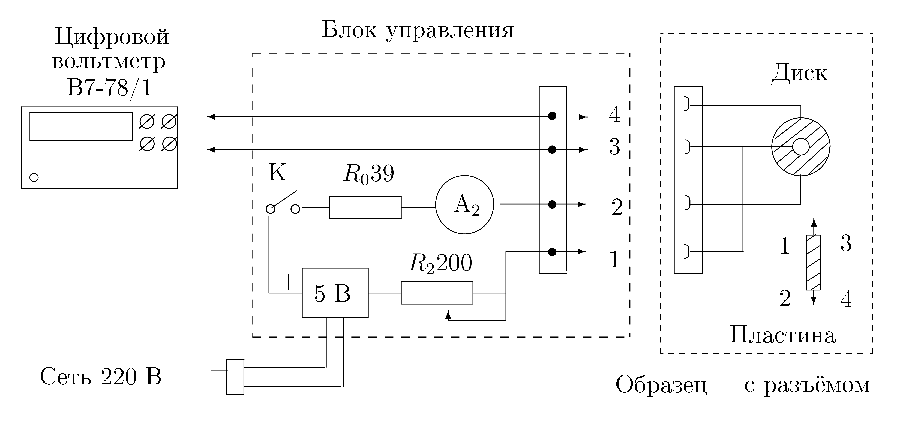
\includegraphics[width = 0.21\textwidth]{Pct1}
\captionsetup{justification = centering}
\caption{Векторная диаграмма\label{Fig1}}
\end{wrapfigure}

Из выражений (\ref{uca}) и (\ref{pca}) можно выразить добротность контура через параметры АЧХ и ФЧХ: пусть $\Delta\omega$ - ширина резонансного пика при напряжении, в $\sqrt{2}$ раз меньшем резонансного. Эту же величину можно получить как разность циклических частот между точками ФЧХ, где $\varphi$ принимает значения $-\frac{\pi}{4}$ и $-\frac{3\pi}{4}$. Примем также за $k$ коэффициент наклона графика ФЧХ в точке резонанса, тогда
\begin{equation}
Q = \frac{\omega_0}{\Delta\omega} = -\frac{k\omega_0}{2}.\label{Q1}
\end{equation}
\paragraph{Поправка к резонансной частоте.} Истинное значение циклической частоты, при которой $U_C$ максимально, отлично от $\omega_0$. Получим для нее более точное выражение, учитывая ранее принятые предположения. Пренебрежем $R_S$ в формуле $(\ref{uc})$, тогда производная $\frac{dU^2_C}{df}$ примет вид
\begin{equation}
\frac{dU^2_C}{df}=\frac{\frac{4\omega}{\omega^2_0}-\frac{2\omega}{Q^2\omega_0^2}-\frac{4\omega^3}{\omega^4_0}}{\frac{1}{Q^2}\left(\frac{\omega}{\omega_0}\right)^2 + \left(\left(\frac{\omega}{\omega_0}\right)^2-1\right)^2}.
\end{equation}
При максимальном напряжении значение этого выражения должно быть равно нулю, исходя из этого несложно получить выражение для $\omega$:
\begin{equation}
\omega = \omega_0\sqrt{1-\frac{1}{2Q^2}}\approx\omega_0\left(1-\frac{1}{4Q^2}\right)\label{omp}.
\end{equation}
\paragraph{Зависимость $R_L$ от частоты.} При достаточно больших частотах активное сопротивление катушки индуктивности может довольно сильно отличаться от значения при постоянном токе. У этого явления есть несколько причин, как то потери энергии за счет наведенных токов в сердечнике, а также потери при перемагничивании, и скин-эффект. Потери энергии за счет перемагничивания дают сопротивление, пропорциональное $\omega$, а за счет наведенных токов - $\omega^2$. Толщина скин-слоя зависит от частоты как $\frac{1}{\sqrt{\omega}}$, а значит сопротивление пропорционально $\sqrt{\omega}$. Таким образом, можно ожидать, что
\begin{equation}
R_L = a + b\sqrt{\omega} + c\omega + d\omega^2\label{rl}.
\end{equation}
\section{Измерение резонансных частот для разных емкостей}
\begin{wrapfigure}{r}{0.47\textwidth}
\centering\includegraphics[width = 0.45\textwidth]{Pct2}
\captionsetup{justification = centering}
\caption{Схема установки\label{Fig2}}
\end{wrapfigure}
\paragraph{Экспериментальная установка.} Схема экспериментальной установки представлена на рис. \ref{Fig2}. С помощью вольтметров мы можем измерять действующие значения напряжения на источнике и конденсаторе, частота $f$ определяется источником. Осциллограф позволяет получить более детальную картину колебаний. Емкость можно изменять с помощью магазина емкостей.

Заметим, что если в предыдущих формулах заменить все амплитуды на действующие значения  (далее будем использовать прежние обозначения для действующих значений), величины $\frac{\omega}{\omega_0}$ на $\frac{f}{f_0}$ ($f_0$ - резонансная частота), а величины $\omega$ на $2\pi f$, то они останутся верными. Поэтому из (\ref{redef}), (\ref{uca}) и (\ref{redef2}) индуктивность выражается по формуле
\begin{equation}
L = \frac{1}{4\pi^2 f_0^2 C}\label{ind},
\end{equation}
где $f_0$ - резонансная частота, добротность по формуле 
\begin{equation}
Q = \frac{{U_C}_0}{E}\label{q},
\end{equation}
где ${U_C}_0$ - действующее значение напряжение в резонансе,  сопротивление по формуле
\begin{equation}
R_\Sigma = \frac{E}{{U_C}_0}\sqrt{\frac{L}{C}}\label{rsig},
\end{equation}
действующее значение тока в цепи по формуле 
\begin{equation}
I = \frac{E}{R_\Sigma}.
\end{equation}
Кроме этого, введем дополнительно следующие параметры:
\begin{equation}
\begin{cases}
\rho = \sqrt{\frac{L}{C}}\text{ - реактивное (или волоновое) сопротивление контура};\\
{R_S}_\text{max} = 10^{-3}\rho\text{ - максимальное активное сопротивление конденсатора}\label{redef3}.\\
\end{cases} 
\end{equation}
В выражении для ${R_S}_\text{max}$ множитель $10^{-3}$ был выбран, т.к. для используемых конденсаторов $\tg\delta \le 10^{-3}$, и в силу выражения
\begin{equation}
R_S = \rho\tg\delta
\end{equation} 
Также, если дополнительно предположить, что $R$ мало меняется с частотой, то, в силу малости $R_S$, из (1) получим
\begin{equation}
R_L = R_\Sigma - R.\label{rle}
\end{equation}

В этой части мы будем снимать зависимость $f_0$ и ${U_C}_0$ от $C$ при неизменном действующем значении напряжения на источнике:
\begin{equation} 
E = (0,100\pm0,001)~\text{В}.
\end{equation}
Значение сопротивления резистора:
\begin{equation}
R = 3,45~\text{Ом}.
\end{equation}
\begin{table}[ht]\centering
\begin{tabular}{|*{8}{c|}}
\hline
$C, ~\text{нФ}$&25,0&33,2&47,5&57,0&67,4&82,1&99,6\\
\hline
$f_0, ~\text{кГц}$&31,5&27,3&23&21,1&19,4&17,6&16\\
\hline
${U_C}_0, ~\text{В}$&2,60&2,33&2,02&1,87&1,75&1,60&1,48\\
\hline
$E, ~\text{В}$&0,100&0,100&0,100&0,100&0,100&0,100&0,100\\
\hline
$L, ~\text{мГн}$&1,02&1,02&1,01&1,00&1,00&1,00&0,99\\
\hline
$\Delta L, ~\text{мГн}$&0,01&0,01&0,01&0,01&0,01&0,01&0,01\\
\hline
$R_{\Sigma}, \text{Ом}$&7,69&7,45&7,18&7,08&6,96&6,90&6,77\\
\hline
$R_L, \text{Ом}$&4,24&4,00&3,73&3,63&3,51&3,45&3,32\\
\hline
$\Delta R_L, \text{Ом}$&0,05&0,05&0,05&0,05&0,05&0,06&0,06\\
\hline
$Q$&26,0&23,3&20,2&18,7&17,5&16,0&14,8\\
\hline
$\rho, \text{Ом}$&200&174&145&132&122&110&100\\
\hline
${R_S}_\text{max}, \text{Ом}$&0,200&0,174&0,145&0,132&0,122&0,110&0,100\\
\hline
$I, \text{мА}$&13,0&13,4&13,9&14,1&14,4&14,5&14,8\\
\hline
\end{tabular}
\caption{Зависимость ${U_C}_0$ и $f_0$ от $C$}
\end{table}
\paragraph{Обработка результатов.} Экспериментальные данные представлены в таблице 1.
Погрешность $f_0$ в силу неточности определения резонансной частоты была принята
\begin{equation}
\Delta f_0 = 0,1~\text{кГц},
\end{equation}
погрешность ${U_C}_0$
\begin{equation}
\Delta {U_C}_0 = 0,01~\text{В}.
\end{equation}
Погрешность $L$, исходя из (\ref{ind}), вычислялась по формуле
\begin{equation}
\Delta L = 2\frac{\Delta f_0}{f_0}\label{dell},
\end{equation}
т.к мы считаем значение емкости точным. Из данных таблицы можно получить среднее значение $L$ (в дальнейшем будем обозначать $L$ именно его), и случайную погрешность $\sigma_L$:
\begin{equation}
L \approx 1,00~\text{мГн};
\end{equation}
\begin{equation}
\sigma_L \approx 5\cdot10^{-3}~\text{мГн}.
\end{equation}
Как мы видим, систематическая погрешность больше случайной, поэтому для дальнейших вычислений принималось:
\begin{equation}
\Delta L = 0,01~\text{мГн}.
\end{equation}
Погрешность $R_L$ вычислялась по формуле
\begin{equation}
\Delta R_L = R_l\sqrt{\left(\frac{\Delta {U_C}_0}{{U_C}_0}\right)^2 + \frac{1}{4}\left(\frac{\Delta L}{L}\right)^2},
\end{equation}
это выражение было получено из (\ref{rsig}), т.к. из (\ref{rle})
\begin{equation}
\Delta R_L = \Delta R_\Sigma,
\end{equation}
при этом мы считали, что значение $R$ известно с достаточной точностью.

График зависимости $R_L(f)$ представлен на рис. 3. На нем представлены фитирования экспериментальных данных двумя зависимостями: вида (\ref{rl}) и вида
\begin{equation}
R_L = a + b\sqrt{f},
\end{equation}
т.е. модели, когда отсутствует сердечник и скин-эффект влияет на всю цепь, в том числе и на $R$. Первая модель обозначена mod1, вторая - mod2.

\begin{wrapfigure}{r}{0.55\textwidth}
\centering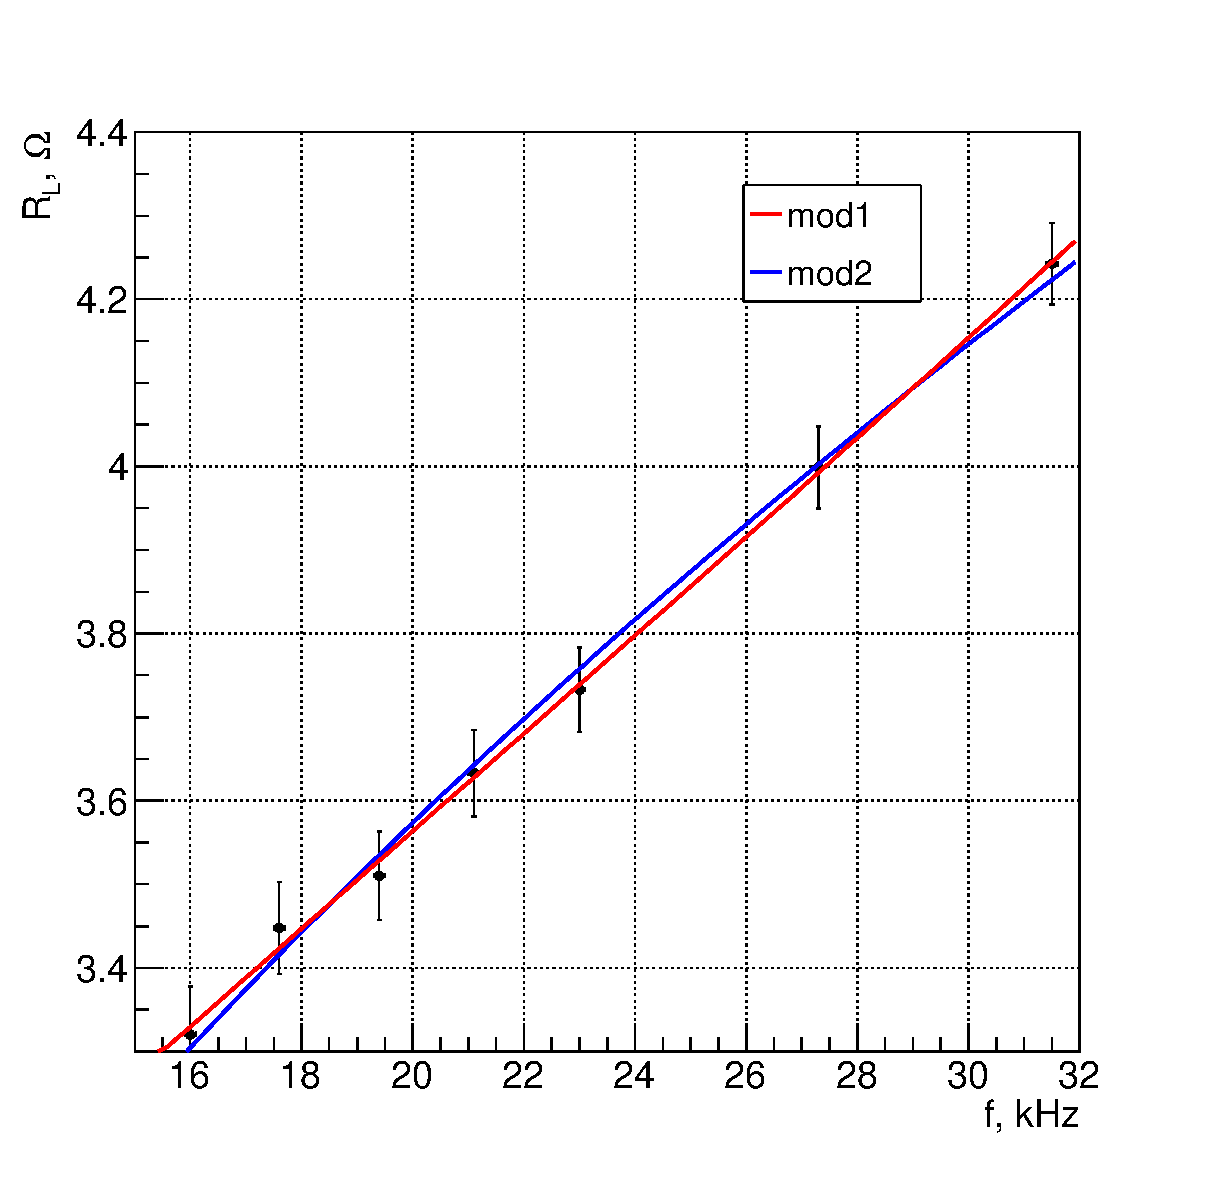
\includegraphics[width = 0.52\textwidth]{Plt1}
\captionsetup{justification = centering}
\caption{График зависимости $R_L(f)$\label{Fig3}}
\end{wrapfigure}

Из графика видно, что точки лежат почти на одной прямой, поэтому для точного определения характера зависимости необходимы измерения в более широком диапазоне. Рассмотрим значения $\chi^2$ для 1 и 2 моделей:
\begin{equation}
\chi_1^2\approx0,38;
\end{equation}
\begin{equation}
\chi_2^2\approx1,06,
\end{equation}
отсюда модель 2 более вероятна, т.к. $\chi^2$ ближе к 1. Поэтому катушка скорее всего не имеет сердечника, и все обусловлено скин-эффектом. Толщина скин-слоя на частоте 10кГц равна
\begin{equation}
\Delta \approx 0,66~\text{мм},
\end{equation}
что довольно мало, поэтому скин-эффект в данном случае существенный.
\section{Измерение АЧХ и ФЧХ}
\begin{wrapfigure}{r}{0.36\textwidth}
\centering\includegraphics[width = 0.33\textwidth]{Pct4}
\captionsetup{justification = centering}
\caption{Возможный вид осциллограммы\label{Fig4}}
\end{wrapfigure}

\paragraph{Экспериментальная установка.} В этой части экспериментальная установка такая же, как и в предыдущей. Вместо настоящего значения фазы $\varphi_C$ будем использовать $|\varphi_C|$, т.к. из формулы (\ref{phic}) следует, что $\varphi_C < 0$, и подобная замена просто изменит знак. Для измерения $|\varphi_C|$ синхронизация первого осциллографа была настроена на первый канал (источник), тогда осциллограмма выглядит примерно как на рис. 4. При использовании параметров, указанных на рисунке (они измеряются в делениях шкалы, т.к. нам нужно только отношение), формула для $|\varphi_C|$ примет вид
\begin{equation}
|\varphi_C| = \pi\frac{x}{x_0}\label{pcee}.
\end{equation}
Измерения проводились при двух разных значениях емкости: 25,0 нФ и 47,5 нФ.
\begin{table}[ht]\centering
\begin{tabular}{|*{9}{c|}}
\hline
$U_C, \text{В}$&0.62&1.14&1.19&1.43&1.85&2.10&2.19&2.42\\
\hline
$f, \text{кГц}$&28.91&30.28&30.31&30.57&30.87&31.02&31.06&31.20\\
\hline
$x, \text{дел}$&0.9&1.0&1.1&1.4&1.9&2.2&2.4&2.9\\
\hline
$x_0, \text{дел}$&8.4&8.2&8.2&8.2&8.1&8.0&8.0&8.0\\
\hline
$\varphi$&0.34&0.38&0.42&0.54&0.74&0.86&0.94&1.14\\
\hline
$\Delta\varphi$&0.04&0.04&0.04&0.04&0.04&0.04&0.04&0.04\\
\hline
$\frac{f}{f_0}$&0.918&0.962&0.963&0.971&0.981&0.985&0.987&0.991\\
\hline
$\Delta \frac{f}{f_0}$&0.001&0.001&0.001&0.001&0.001&0.001&0.001&0.001\\
\hline
$\frac{U_C}{U_0}$&0.238&0.438&0.458&0.550&0.712&0.808&0.842&0.931\\
\hline
$\Delta \frac{U_C}{U_0}$&0.004&0.004&0.004&0.004&0.005&0.005&0.005&0.005\\
\hline
$U_C, \text{В}$&2.51&2.60&2.57&2.32&1.94&1.52&1.14&0.63\\
\hline
$f, \text{кГц}$&31.30&31.44&31.53&31.75&32.01&32.32&32.73&33.86\\
\hline
$x, \text{дел}$&3.3&3.8&4.1&5.0&5.5&6.0&6.3&6.5\\
\hline
$x_0, \text{дел}$&7.9&7.9&7.9&7.8&7.8&7.7&7.6&7.5\\
\hline
$\varphi$&1.31&1.51&1.63&2.01&2.22&2.45&2.60&2.72\\
\hline
$\Delta\varphi$&0.04&0.04&0.04&0.05&0.05&0.05&0.05&0.06\\
\hline
$\frac{f}{f_0}$&0.994&0.999&1.002&1.009&1.017&1.027&1.040&1.076\\
\hline
$\Delta \frac{f}{f_0}$&0.001&0.001&0.001&0.001&0.001&0.001&0.001&0.001\\
\hline
$\frac{U_C}{U_0}$&0.965&1.000&0.988&0.892&0.746&0.585&0.438&0.242\\
\hline
$\Delta \frac{U_C}{U_0}$&0.005&0.005&0.005&0.005&0.005&0.004&0.004&0.004\\
\hline
\end{tabular}
\caption{Данные для получения АЧХ и ФЧХ при $C = 25,0~\text{нФ}$}
\end{table}
\begin{table}[!ht]\centering
\begin{tabular}{|*{9}{c|}}
\hline
$U_C, \text{В}$&0.59&0.93&1.19&1.43&1.62&1.77&1.93&1.99\\
\hline
$f, \text{кГц}$&21.16&21.98&22.31&22.52&22.65&22.76&22.89&22.97\\
\hline
$x, \text{дел}$&0.5&0.7&0.9&1.1&1.3&1.5&1.7&1.9\\
\hline
$x_0, \text{дел}$&4.7&4.6&4.5&4.5&4.4&4.4&4.4&4.4\\
\hline
$|\varphi_C|$&0.33&0.48&0.63&0.77&0.93&1.07&1.21&1.36\\
\hline
$\frac{f}{f_0}$&0.92&0.95&0.97&0.97&0.98&0.99&0.99&0.99\\
\hline
$\Delta|\varphi_C|$&0.067&0.069&0.071&0.072&0.074&0.075&0.077&0.078\\
\hline
$\Delta \frac{f}{f_0}$&0.001&0.001&0.001&0.001&0.001&0.001&0.001&0.001\\
\hline
$\frac{U_C}{U_0}$&0.292&0.460&0.589&0.708&0.802&0.876&0.955&0.985\\
\hline
$\Delta \frac{U_C}{U_0}$&0.005&0.005&0.006&0.006&0.006&0.007&0.007&0.007\\
\hline
$U_C, \text{В}$&2.01&1.98&1.84&1.60&1.27&0.95&0.74&0.46\\
\hline
$f, \text{кГц}$&23.06&23.16&23.34&23.53&23.80&24.16&24.56&25.47\\
\hline
$x, \text{дел}$&2.1&2.3&2.7&3.0&3.3&3.5&3.5&3.6\\
\hline
$x_0, \text{дел}$&4.3&4.3&4.3&4.3&4.2&4.2&4.1&3.9\\
\hline
$|\varphi_C|$&1.53&1.68&1.97&2.19&2.47&2.62&2.68&2.90\\
\hline
$\frac{f}{f_0}$&1.00&1.00&1.01&1.02&1.03&1.05&1.06&1.10\\
\hline
$\Delta|\varphi_C|$&0.081&0.083&0.086&0.089&0.095&0.097&0.101&0.110\\
\hline
$\Delta \frac{f}{f_0}$&0.001&0.001&0.001&0.001&0.001&0.001&0.001&0.001\\
\hline
$\frac{U_C}{U_0}$&0.995&0.980&0.911&0.792&0.629&0.470&0.366&0.228\\
\hline
$\Delta \frac{U_C}{U_0}$&0.007&0.007&0.007&0.006&0.006&0.005&0.005&0.005\\
\hline
\end{tabular}
\caption{Данные для получения АЧХ и ФЧХ при $C = 47,5~\text{нФ}$}
\end{table}

\paragraph{Обработка результатов.} Экспериментальные данные представлены в таблицах 2 и 3 - для 25,0 нФ и 47,5 нФ соответственно. Измерения $f$ считались точными (погрешность прибора с учетом случайных отклонений 10 Гц, что очень мало). Погрешность $U_C$ принималась равной
\begin{equation}
\Delta U_C = 0,01\text{В},
\end{equation}
погрешности $x$ и $x_0$ 
\begin{equation}
\Delta x = \Delta x_0 = 0,1\text{дел}.
\end{equation}
Погрешность $\Delta\varphi$, исходя из (\ref{pcee}), оценивалась по формуле
\begin{equation}
\Delta|\varphi_C| = |\varphi_C|\sqrt{\left(\frac{\Delta x}{x}\right)^2 + \left(\frac{\Delta x_0}{x_0}\right)^2},
\end{equation}
погрешность $\frac{f}{f_0}$ - по формуле
\begin{equation}
\Delta\frac{f}{f_0} = \frac{f}{f_0}\frac{\Delta f_0}{f_0},
\end{equation}
здесь значение $\frac{\Delta f_0}{f_0}$ можно получить из \ref{omp}:
\begin{equation}
\frac{\Delta f_0}{f_0} \approx \frac{1}{4Q^2} \approx 0,001,
\end{equation}
как будет показано в дальнейшем. Погрешность $\Delta\frac{U_C}{{U_C}_0}$ определялась по формуле
\begin{equation}
\Delta\frac{U_C}{{U_C}_0} = \sqrt{\left(\frac{\Delta U_C}{U_C}\right)^2 + \left(\frac{\Delta {U_C}_0}{{U_C}_0}\right)^2}. 
\end{equation}

\begin{wrapfigure}{rh!}{0.54\textwidth}
\centering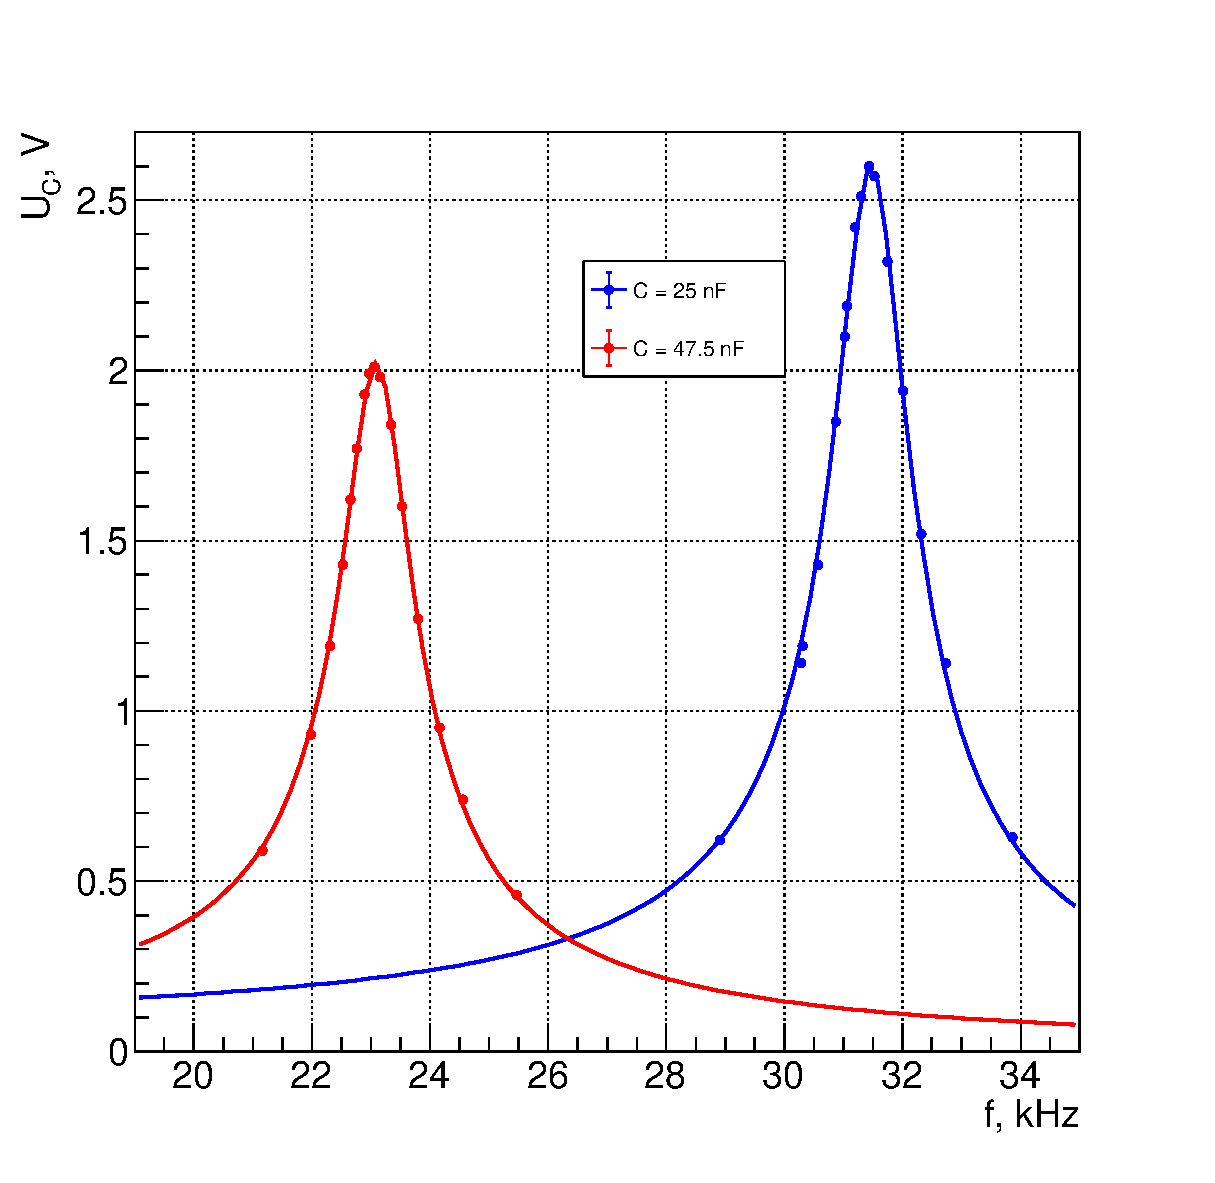
\includegraphics[width = 0.53\textwidth]{Plt2}
\captionsetup{justification = centering}
\caption{График зависимости $U_C(f)$\label{Fig5}}
\vspace{25pt}
\end{wrapfigure}

Графики зависимости $U_C(f)$ представлены на рис. 5. Данные были профитированы зависимостью (6) с учетом того, что
\begin{equation}
\omega = 2\pi f.
\end{equation}
Как мы видим, экспериментальные данные хорошо легли на эту зависимость, хотя коэффициенты $\chi^2$ получились довольно большие (122 для 25,0 нФ и 36 для 47,5 нФ), что, скорее всего, вызвано недооценкой ошибки. Параметры зависимости для 25,0 нФ:
\begin{equation}
f_0 = (31,480\pm0,002)~\text{кГц};
\end{equation}
\begin{equation}
Q = 26,02\pm0,05.
\end{equation}
Как мы видим, значение $Q$ совпадает со значением из предыдущей части. Значение $R_S$ получилось равным
\begin{equation}
R_S = (0\pm12)~\text{Ом},
\end{equation} 
таким образом, определить $R_S$ в данном эксперименте невозможно (но это сопротивление мало), поэтому в дальнейшем это сопротивление не указывается. Для 47,5 нФ получились следующие параметры:
\begin{equation}
f_0 = (23,100\pm0,002)~\text{кГц};
\end{equation}
\begin{equation}
Q = 20,02\pm0,13,
\end{equation}
что также совпадает с данными предыдущих пунктов. Для построения последующих графиков были использованы полученные значения $f_0$, в качестве погрешности была взята величина
\begin{equation}
\frac{1}{4Q^2}\sim\frac{1}{4\cdot20^2}\approx0,01,
\end{equation}
как и было в (42).

График зависимости $|\varphi_C|\left(\frac{f}{f_0}\right)$ представлен на рис. 6. Функция для фитирования была получена из (\ref{phic}) с учетом (44) и преобразования
\begin{equation}
f = \frac{f}{f_0}f_0.
\end{equation}
\begin{wrapfigure}{rh!}{0.55\textwidth}
\centering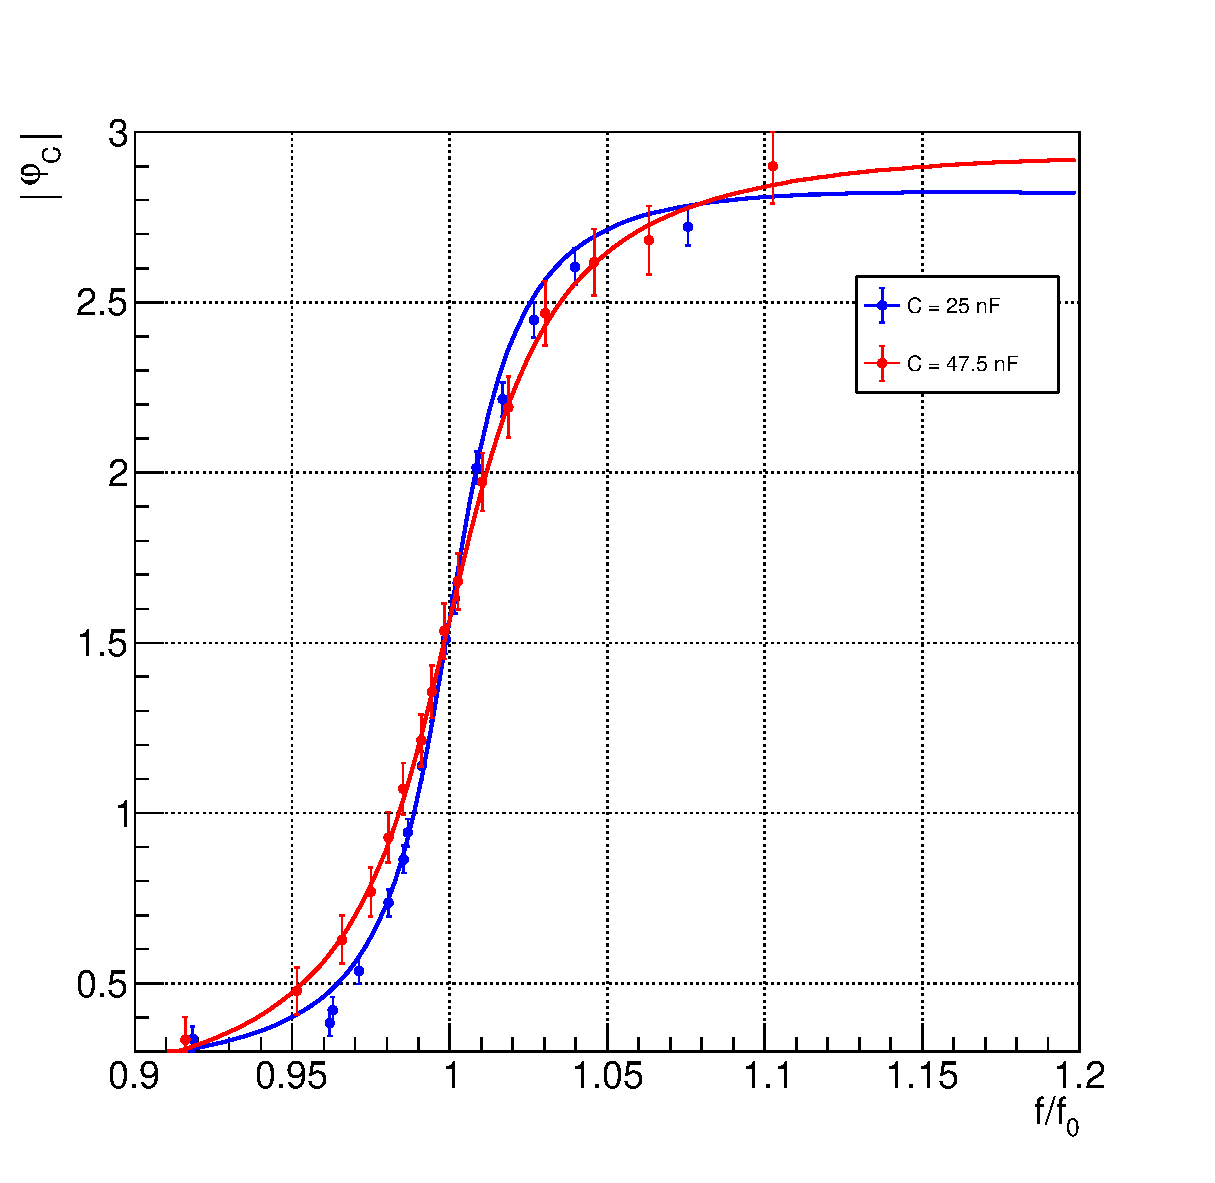
\includegraphics[width = 0.53\textwidth]{Plt3}
\captionsetup{justification = centering}
\caption{График зависимости $|\varphi|\left(\frac{f}{f_0}\right)$\label{Fig6}}
\end{wrapfigure}
Эти данные хуже совпадают с полученными зависимостями, чем данные $U_C(f)$, но относительные погрешности в данном случае также больше. Тем не менее, коэффициенты $\chi^2$ здесь ближе к 1 (1,2 для 47,5 нФ и 18 для 25,0 нФ). Такой большой коэффициент для 25,0 нФ связан, скорее всего, с плохими измерениями. Для 25,0 нФ добротность (теперь в фитировании только 2 параметра - $Q$ и $R_S$) равна
\begin{equation}
Q = 30\pm2,
\end{equation}
что близко к полученным ранее значениям, но не совпадает с ними, что еще раз подтверждает предположение о плохих измерениях. Для 47,5 нФ добротность равна
\begin{equation}
Q = 20\pm2,
\end{equation}
что совпадает с предыдущими значениями.

График зависимости $\frac{U_C}{{U_C}_0}\left(\frac{f}{f_0}\right)$ представлен на рис. 7. Для пересчета были использованы значения ${U_C}_0$, полученные из фитирования зависимости $U_C(f)$:
\begin{equation}
\begin{cases}
{U_C}_0 = (2,61\pm0,01)~\text{В}\text{ - для 25,0 нФ};\\
{U_C}_0 = (2,02\pm0,01)~\text{В}\text{ - для 47,5 нФ}.\\
\end{cases}
\end{equation}
\begin{wrapfigure}{r}{0.55\textwidth}
\vspace{-25pt}
\centering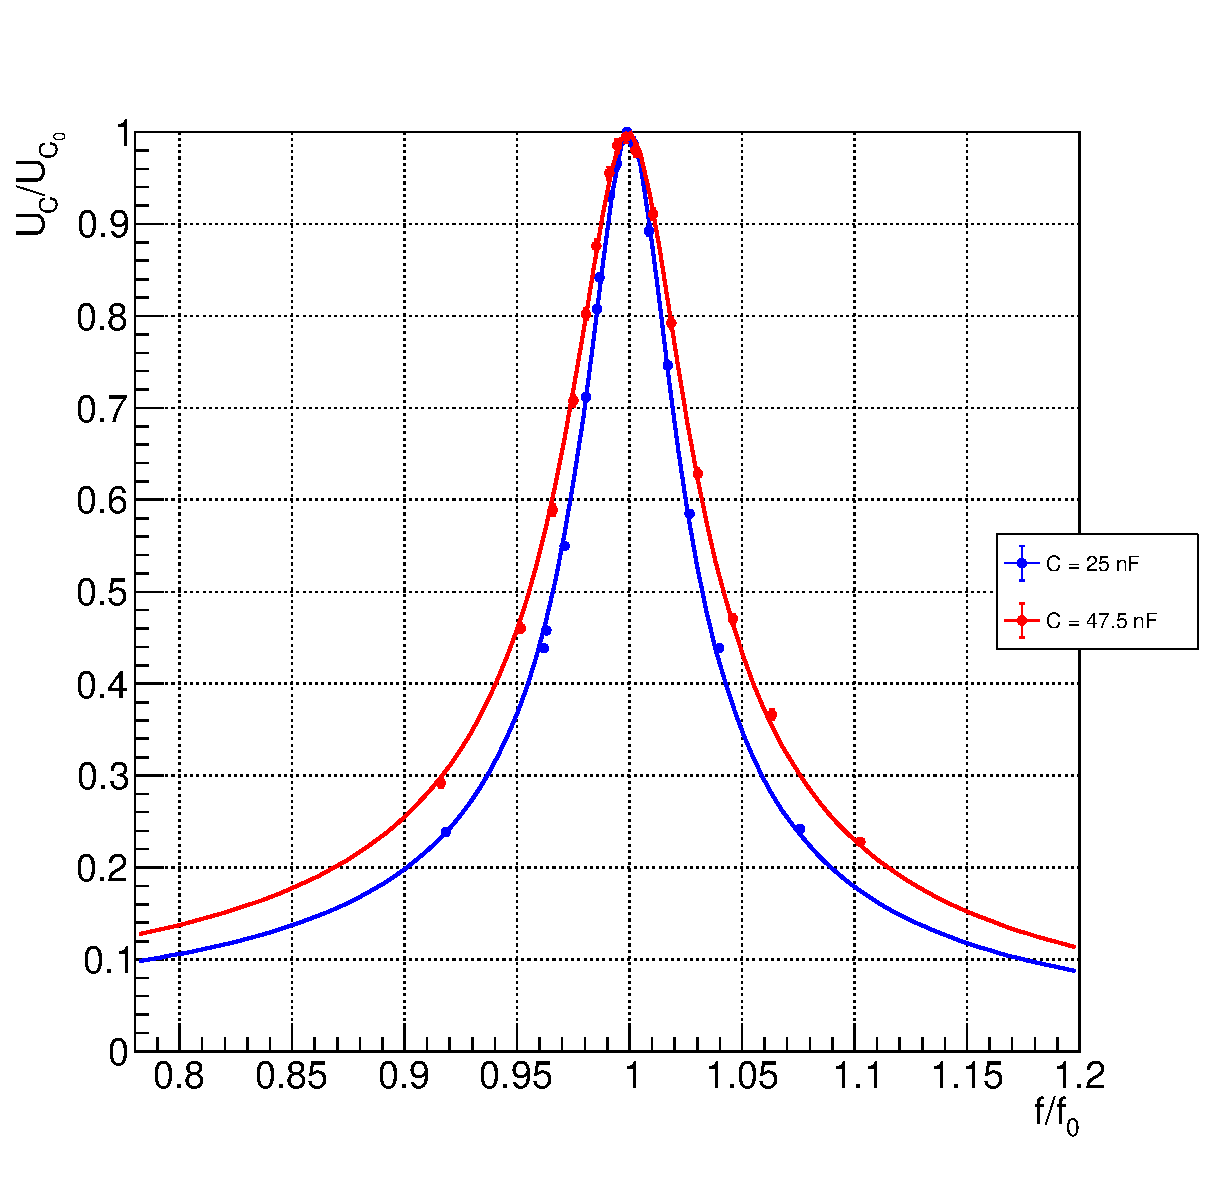
\includegraphics[width = 0.53\textwidth]{Plt4}
\captionsetup{justification = centering}
\caption{График зависимости $\frac{U_C}{{U_C}_0}\left(\frac{f}{f_0}\right)$\label{Fig7}}
\vspace{-15pt}
\end{wrapfigure}
Здесь экспериментальные данные хорошо совпадают с зависимостью, но и коэффициенты $\chi^2$ большие (13 для 25,0 нф  и 11 для 47,5 нФ). Параметрами также были только $R_S$ и $Q$, значение добротности для 25,0 нФ:
\begin{equation}
Q = 26,1\pm0,2,
\end{equation}
что хорошо совпадает с предыдущими данными. Добротность для 47,5 нФ:
\begin{equation}
Q = 20,1 \pm 0,1,
\end{equation}
что также хорошо согласуется с ранее полученными данными.

\section{Векторная диаграмма}
Построим векторную диаграмму напряжений и токов в резонансном состоянии при минимальной добротности (т.е. при $C = 99,6~\text{нФ}$). Сдвиг фаз между напряжениями на источнике и конденсаторе равен $-\frac{\pi}{2}$, между напряжением на источнике и на катушке $\frac{\pi}{2}$. Соответствующие действующие значения напряжений (в резонансе амплитуда напряжения на катушке равна амплитуде напряжения на конденсаторе) и тока можно найти в таблице 1. С учетом того, что амплитуды в $\sqrt{2}$ больше действующих значений, на рис. 8 была построена соответствующая векторная диаграмма. Подписи осей указаны в вольтах, т.к. вектор тока только один, то нет смысла вводить масштаб для силы тока.
\section{Заключение}
\begin{wrapfigure}{r}{0.3\textwidth}
\psfrag{U}[c][c]{$U_L$}
\psfrag{UC}{$U_C$}
\centering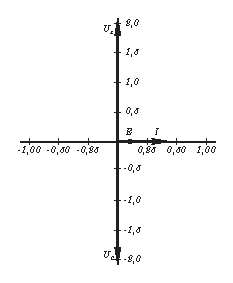
\includegraphics[width = 0.27\textwidth]{Pct5.eps}
\captionsetup{justification = centering}
\caption{Векторная диаграмма для $C = 99,6~\text{нФ}$\label{Fig8}}
\end{wrapfigure}
Цели работы были достигнуты, определена индуктивность контура и получена зависимость его сопротивления от частоты, хотя и в узком диапазоне. Кроме этого, значение добротность для двух емкостей получено несколькими разными способами, а именно по формуле и через графики АЧХ и ФЧХ, и получившиеся значения совпали. Также была построена векторная диаграмма для контура с самой низкой добротностью в резонансном состоянии.
\end{document}